\documentclass[journal]{./IEEEtran}
\usepackage{graphicx}
\usepackage{multirow}
\usepackage{url}
\usepackage{cite}

\begin{document}
\title{Grandmaster Story}

%% Substitions for anything not completely decided 
\newcommand{\sysname}{Grand Master Story}

\author{\IEEEauthorblockN{Nick~Feeney,
Mike~Buerli,
Eric~Buckthal,
and Connor~Lange}\\
\IEEEauthorblockA{Computer Science Department\\
California Polytechnic State University\\
San Luis Obispo, CA\\
\url{{ndfeeney,rclange,mbuerli,ebucktha}@calpoly.edu}}}

\maketitle

\begin{abstract}

In this paper we explore the possibility of using chess games to generate stories. We built a chess game parsing system that could read in and track chess games from the standard PGN format. Next, we defined eleven features which we believed described the state of the game over a set of moves. Using these features we attempted to generate stories based on the chess game through the use of handcrafted story skins. To accomplish the story generation we build a plot tree iterator that was able to handle, text replacement, plot tree iteration, and resources management. We were able to generate fairly good stories that utilized the chess game to determine the plot of the story. Depending on the chess game different events would happen in the plot. Unfortunately, we found that to have the plot of the story closely match the events of the chess game the input story skin needed to be very detailed with many plot nodes. As of now a detailed story skin requires a large amount of human input.

\end{abstract}

\begin{IEEEkeywords}
story generation, drama analysis
\end{IEEEkeywords}

\section{Introduction}
Story generation and drama management have explored many fields to attempt to create interactive and interesting drama. The goal of drama management systems is to organize a particular narrative to reflect particular actions of a user; the drama manage often attempts to steer drama in a particular way or change the environment, characters, plot as if the story was being told by a human watching the same events. If a drama manager prefers to have his subjects follow a more specific story arc, the range of actions a user can perform to influence the system are limited. On the other hand, if a system prefers an open-ended environment with many possible plot events and story outcomes it is possible to allow users to choose their own fate. Human emotion and character development is another focused aspect of story mediation. Some systems interpret how the player converses with characters in the game and the game reacts.
Because our interface for story generation is chess, the control the user has over the course of the story has an interesting aspect--there are a limited set of possible moves the player can provide and there is no set translation from chess moves to story features. Chess has complex strategy in which player advantages and intentions are not easily inferred. The goal of this project was to explore the possibility of utilizing chess games to automatically generate stories. We theorised that events that transpire during a chess game could be translated into plot points which could be then combined to create a narrative plot. Our solution is comprised of five main sections, chess game parsing, chess game state reconstruction, chess move feature extraction, story plot iterator, and finally story skins.
First, we built a PGN chess game parsing system that we used to parse meta data and chess moves from chess games we obtained from the internet. Next, we built a system that could keep track of the current state of the chess board after every chess move. We needed this system because the PGN file format does not include information about the current state of the game it simply lists the moves made during the chess game. We then created a list of eleven features that could be pulled out of a series of chess moves. These features ranged from how dramatic a move was to how far a piece traveled in a set of moves. Next, we built a story plot iterator that assigned chess moves to story plot nodes and then generated text that was bound together to form our stories. To generate the text for a plot node we created a story skin system. These skins were responsible for the text generation. Each skin was capable of utilized text replacement as well as resource management to generate text blocks. In the solution section we go into more detail about how each piece works, for an overall system design see Figure~\ref{sysoverview}.

\begin{figure}[h!]
\begin{center}
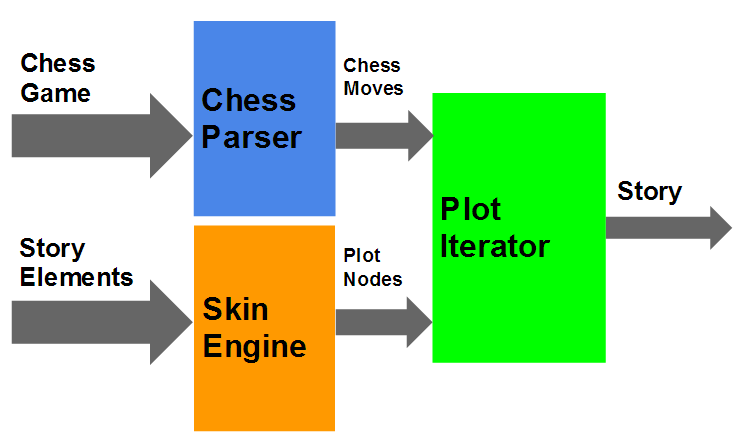
\includegraphics[width=3.0in]{./overview}
\end{center}
\caption{The \sysname{}}
\label{sysoverview}
\end{figure}

\subsection{Paper Layout}
The structure of the rest of the paper is as follows: Section 2 describes previous work, Section 3 explains the details of the \sysname{}, Section 4 analyzes the results of the \sysname{}, Section 5 outlines future work and Section 6 concludes. 

\section{Related Work}

This work was originally founded in the dramatic theory of Vladimir Propp. \cite{Propp68} Propp analyzed Russian folk tales into a specific set of functions--independent plot structures deemed the minimal dramatic step of a story. These functions are understood as an act of a single character, defined with the significance of the course of action. Stemming from the idea of an independent point of plot drama, we evolved to a more open feel because the Propp functions were restricting. Other implementations of Drama Management systems are based heavily on their architecture. 
Interactive Drama Architecture (IDA) \cite{diageng} proposes three key components to interactive drama: the Writer, the Director, and the User. IDA gives the Writer a reasonable amount of control in plot specification, while considering the desire of the User to control how the drama unfolds. IDA is then a first-order logic representation of several components for each scene and they consider the scene as the smallest dramatic moment and the Writer’s goal is to move the story forward as a whole. After a human supplies a loosely constructed plot, the following concept approaches the drama solution:
\begin{itemize} 
\item Annotate each possible object, character, etc. with attributes (whatever they may be) and then heuristically choose the binding for each variable.
\item Have a default binding for each variable. This would put more work on the designer, but at the same time would allow the Designer to input an instantiation of the story as the default.
\item Randomly choose a binding. The Director then still retains control of encouraging characters to perform certain actions such as ending the scene.
\end{itemize}
In Search-Based Drama Management (SBDM) \cite{sbdm}, a player’s concrete experience in the world is captured by a sequence of Player Moves, abstract plot points that a player’s activity can cause to happen. A single Player Move may encapsulate 5 or 10 minutes of concrete player activity in the world - moving around, picking up objects, interacting with characters and so forth. When the concrete activity “adds up” to a story significant event, then a Player Move is recognized. A SBDM has a set of System Moves available that can materially alter the world (e.g. move objects around, change goals in characters’ heads, etc.) in such a way as to encourage or obviate a Player Move. System Moves give the SBDM a way to warp the world around the player so as to make certain Player Moves more or less likely. Besides the System Moves, the author also provides the SBDM with a story specific evaluation function that, given a complete sequence of Player and System Moves, returns a number indicating the “goodness” of the story. Whenever the drama manager recognizes a Player Move (plot point) occurring in the world, it projects all possible future histories of Player and System moves, evaluates the resulting total histories with the evaluation function, and backs these evaluations up the search tree (in a manner similar to game-tree search) to decide which system move to make next that is most likely to cause a good total story to happen.
Declarative Optimization-based Drama Management (DODM) focuses on real-time drama integration in video games and it most closely represents the architecture Chess-based Story Generation creates. EMPath \cite{empath} specifically targets a dungeon-style game in which a player is able to explore and complete tasks. The goal is to create a dramatic element to a concrete and playable atmosphere. To configure DODM for a specific world, the author specifies plot points, drama manager actions, and an evaluation function. Plot points are important events that can occur in an experience. Different sequences of plot points define different player trajectories through games or story worlds. Examples of plot points include a player gaining story information or acquiring an important object. 

%% Examples
\subsection{Story Generation}

\subsection{Chess Analysis}

\section{\sysname{} Design and Implementation}

\subsection{Chess Game Extraction} 
To generate stories from chess games, we first needed to obtain a large number of chess games to use as our data set. We gathered 2,367 games from \_\_ in the form of Portable Game Notation (PGN) files. Since each game was in a known format, we simply extracted the information from each game using a regular expression and stored it in a Python dictionary. Each game included the following custom tags, in addition to the standard PGN set \cite{pgntags} and the set of moves in the game:
\begin{itemize} 
\item WhiteELO - the ranking of the white player (not always present)
\item BlackELO - the ranking of the black player (not always present)
\item WhiteCountry - the home country of the white player
\item BlackCountry - the home country of the black player
\item PlyCount - the total number of half-moves played
\end{itemize}

\subsection{Chess Game State Reconstruction} 
The chess moves \_\_ from the chess parser, represent a set state diagram of the chess game. The only information that is given is the type of piece and destination, as well as if there was a capture or some other activity. Iterating through this list of moves, we are able to disambiguate the correct chess piece as well as the starting location of the piece being moved. In this way we can construct a list of chess moves that not only keeps track of the current state of the game and the chess board, but provide features of each individual move. Moves can be further analyzed by calculating features of the game, like the total number of threatened pieces as well as the number of targeted pieces (pieces that can be captured in the next turn). Ultimately the set of chess moves will be grouped by the plot iterator and features will be extracted from groups of moves.

\subsection{Chess Move Feature Extraction}
The features that were developed for this project attempted get a general overview of the effect that the group of chess moves had on the game. The exact effect of a feature on the chess game is entirely dependent on the skin that is provided for the story. The exact way a chess game feature is use is explained in the Plot Iterator section. In the end, there were eleven features, Dramatic, Danger, Hero, Travel, Unimportant Death, Important Death, Unimportant Kill, Important Kill, Check, Safety, and Defeat. 
\begin{itemize}
\item Dramatic was a feature that we used to measure how many pieces that a player had in threat.
\item Danger was a feature that we developed to measure how many pieces that a player owns and are in threat.
\item Hero was a feature that we developed to signal when a single piece takes or kills two or more pieces in a set of moves.
\item Travel was a feature that we used to signal when a large amount of the chessboard was covered by the pieces of a player.
\item Unimportant Death signaled when a pawn was lost.
\item Important Death signaled when a none pawn piece was lost.
\item Unimportant Kill signaled when a pawn was killed.
\item Important Kill signaled when none pawn piece was killed.
\item Check is the feature that signals when a player puts the other player’s king into check.
\item Safety was the feature signalling that a player won the game.
\item Defeat signals when a player lost a game.
\end{itemize}

\subsection{Skins}
\subsubsection{Plot tree}
A plot tree is defined as a set of plot nodes, or happenings, in a given story. In a given skin, the plot is constructed by a list of plot nodes that each contain a list of indices, describing the set of next possible plot nodes. In this way we can map plot happenings, restricting linear portions of a story’s plot, while also modeling multiple plot branches. This architecture also allows for plot nodes to link back to previous nodes. An example of what a plot tree may look like for a given story is shown in Figure~\ref{plotree}

\begin{figure}[h!]
\begin{center}
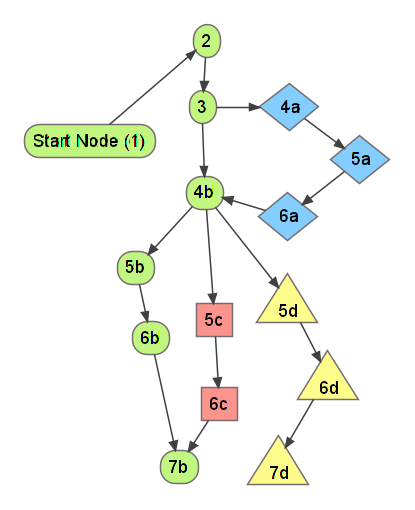
\includegraphics[width=3.0in]{./plotTree}
\end{center}
\caption{The \sysname{} Plot Tree}
\label{plotree}
\end{figure}


\subsubsection{Plot node}
A plot node is the fundamental unit of the plot graph. It includes templates, all features associated with the template(s), resources associated with the node, wordsets used for populating the templates, and a list of nodes in the plot graph that are reachable from this node. Each plot node also contains a generateText() method that populates the chosen template with selected words from the template's wordset. 

Text generation is done by selecting a random template from the list of template and doing tag replacement. Tag replacement is done recursively, replacing tags within tags with random choices from the skin’s wordset. While replacing tags, the plot node also keeps track of resources used, deleting a resource word or tag if it is used in a sentence. Lastly after a template has been converted into a sentence, or sequence of sentences, the template used is removed from the list. Once a plot node runs out of templates, the plot iterator can no longer branch to that specific node. This allows for two levels of randomness, both on the sentence level and the word level while never repeating the same template twice.

In addition to methods that populate the story, the plot node class also contains methods to determine properties of the plot graph such as shortest distance from the current node to a node that concludes the story and the maximum depth of the plot tree. These properties are ultimately used during the story generation phase of \sysname{} to ensure the constructed story matches the chess game.

\subsubsection{Templating}
The story skin contains a list of lists of templates that are associated with each plot node. Templates are patterns or structures that form a sentence or group of sentences. They are put together like a normal sentence, however with words and phrases replaced by tags. Tags are defined as words(alpha-numeric) that begin with an ‘@‘ character. These words or phrases are replaced at runtime with words or phrases from the corresponding tag in the wordset. Tags can be recursive, with tag mentions within a value for a given tag.

The wordset for a plot is a dictionary constructed from four parts in the skin; words, constants, choices, and resources. Words, the most general type in the wordset, is a dictionary lists for each tag. Each list contains one or more strings, from which one will be randomly chosen for every instance of the tag in the given template. Constants, much like “words”, is also a dictionary of lists. Its main difference is that one string is chosen from the list at the beginning and remains constant throughout a given story. Next, “choices” is a list of tuples that contain tags and options. At the beginning of story generation, the tags are randomly mapped to the option strings, so that no two tags have the same value. This allows for easy assignment of groups of names and objects to tags. Lastly “resources” is a dictionary of tags where strings from each list are deleted once they are used. If all values have been deleted the tag defaults to the “words” set for replacement. 




\subsubsection{Story Skins}
War story - text replacemet
Romeo and Juliet - plot branches
Zombie Story - feature analysis

\subsection{Plot Iterator}
The Plot Iterator is the component of \sysname{} that generates story content from chess move features and a plot graph. Each portion of the iterator is discussed in detail in the following subsections. 

\subsubsection{Chess Move Grouping}
Since most of the games we extracted tended to have upwards of 50 moves in them, we couldn’t map plot nodes (of which there are less than 50) to each individual move in a game. We originally attempted to use aggregate statistics about the game , in conjunction with examining the features of a particular move to determine importance, to influence a weighted drop rate when pruning moves. However, this lead to less than satisfactory results and we ultimately decided to utilize a uniform grouping of moves. The features for each individual move in the grouping are summed to produce the features of the move grouping. 

\subsubsection{Plot Tree Traversal}
The traversal of the plot graph starts with the first plot node, which is fixed for a given skin. The plot iterator then traverses each node one-by-one, calling each node’s generateText() method to build parts of the story, until it gets to a potential branch (either an omission of an event or a different plot path) in the plot graph. To determine which path to take in the plot graph, the iterator calculates the total feature correlation of the move grouping by summing the weights of each feature for each move. Whichever plot node in the graph has the most similar value to the calculated feature weights of the move grouping is chosen. The exact method of calculating feature weights is discussed in the following section. The plot iterator then repeats this process until it gets to the end of the plot graph.

\subsubsection{Finding the Best Marched Feature}
We tried a few different matching algorithms when attempting to match the chess game features with the story skin features. In the end we got the best results with a very simple direct matching method. Our algorithm compared the features of the chess game with the features of the story plot node and found how many overlapped. We then took to overlapping score and subtracted the difference in the total number of features. This method simply favored plot nodes that had the most features in common and had a similar amount of features.

\section{Results}
Need results

\section{Future Work}
This project has many pieces that could be expanded for future work. The most obvious and probably the most worthwhile would be to automate the story skin generation. The main limiting factor of this entire project is that the story skins that are needed to generate new stories are handwritten. If there was a way to automatically generate these skins then better and more varying stories could be generated which would also require much less human input.

Another main area for expansion on this project would be feature extraction. We developed a small but potent feature set. Smaller features or less obvious features could be developed which could add more detail into the stories. Character tracking could also be implemented and provide a plot that matched the chess game more accurately. Character tracking would mean that each chess piece is assigned to a character in the story and the fate of that chess piece would dictate that character’s actions.

\section{Conclusion}
This project was performed to test the validity of generating stories based on the events that transpire in a chess game. Our implementation proves that it is in fact possible but there is still much room for improvement. The chess game parser does a good job parsing the PGN file format. The chess game tracker does a really good job tracking the state of the game. The chess game feature extraction does a good job getting the central themes of the game but could be expanded to get more detailed features. The plot iterator does an excellent job managing the story skins. The current version of the story skins do a good job at generating text but require large amounts of user input to create. As it is now each story skin takes about about two hours to write.  We believe that with a few modifications a similar system will perform extremely well and require much less human input. This topic shows a great deal of potential and hopefully will be expanded in the future.

\section{Acknowledgment}

\bibliographystyle{IEEEtran}
\bibliography{IEEEabrv,./references}

\end{document}

